\newcommand{\assignmentDate}{December 2nd, 2019}
\newcommand{\norm}[1]{\left\lVert#1\right\rVert}
% Add title
%Institute
\begin{tabular*}{\hsize}{l@{\extracolsep{\fill}} r}
	\textsc{Technical University of Berlin}		 \hfill&								 	\\
	Faculty II - Mathematics and Natural Sciences\hfill&									\\
	Institute of Mathematics 					 \hfill&									\\
	Dr. D. Peschka, A. Selahi 		 			 \hfill&									\\
\end{tabular*}

% Title
\begin{center}
	\textbf{\Large{\courseName}}\\
	\vspace{7pt}
	\large{Homework \currentAssignment}\\
	\smallskip
	\normalsize{Submitted on \assignmentDate}
\end{center}

% Group table
\begin{center}
	\vspace{-8pt}
	\begin{tabular}{l c r}
		by \textbf{\groupNumber}		    &	 			  &		 								\\
		\hline
		\texttt{Kagan Atci} 			    & \texttt{338131} & \texttt{Physical Engineering, M.Sc.}\\
		\texttt{Navneet Singh }		 	    & \texttt{380443} & \texttt{Scientific Computing, M.Sc.}\\ 
		\texttt{Daniel V. Herrmannsdoerfer} & \texttt{412543} & \texttt{Scientific Computing, M.Sc.}\\ 
		\hline
	\end{tabular}
\end{center}

% EXERCISE 1
% --------------------------------------------------------------------------------------------------------------------
\addExercise{1}{Ex1}

%
% ----------------
\addSubExercise{a}

%
% ----------------
\addSubExercise{b}

%
% ----------------
\addSubExercise{c}

%
% EXERCISE 2
% --------------------------------------------------------------------------------------------------------------------
\addExercise{2}{Ex2}
%
% ----------------
\addSubExercise{a}
The discrete algorithm is implemented in a similar fashion to the one for section $II.5$ in the script, changing the lexicographic indexing to have the angle $\varphi$ vary over $i$ and $r$ over $j$. The operators are constructed in blocks by using Kronecker products of matrices containing the inverse radius coefficients for $\frac{1}{r_{ij}}\partial_{r}u_{ij}$ and $\frac{1}{r_{ij}^2}\partial_{\varphi\varphi}u_{ij}$. Multiplied with the corresponding adjacency matrices. The part a) and c) are thus jointly implemented in the program \listinline{a06ex02\_getPDE.py}

%
% ----------------
\addSubExercise{b}
We say the finite difference method is consistent if

\begin{equation*}
    \norm{f_h-L_h R_h u}_h \xrightarrow{ h \to 0} 0
\end{equation*}

Wlog let us take the maximum norm, that way we can write, by writing out the action of the restriction operator and the $L_h$ matrix:

\begin{equation*}
    max(f_h-L_hR_hu) \xrightarrow{ h \to 0} 0=
\end{equation*}

So lets consider the particular index $(ij)$ for which the maximal difference is reached, knowing that the difference stencil jumping considering neighbouring indices $j$ is the difference operator with respect to $r$ and the one considering neighbouring $i$ the one for $\varphi$

\begin{equation*}
    |(\partial_{rr}u_{ij}-D^{+}_jD^{-}_j)
    +\frac{1}{r_{ij}}(\partial_{r}u_{ij}-D^{0}_j)
    +\frac{1}{r_{ij}^2}(\partial_{\varphi\varphi}u_{ij}-D^{+}_iD^{-}_i)|
\end{equation*}

By the triangle inequality we can bound the expression by the sum of the maximums and take out the constant factors $\frac{1}{r_{ij}}$ and $\frac{1}{r_{ij}^2}$ since they are always positive.

\begin{equation*}
    |\partial_{rr}u_{ij}-D^{+}_jD^{-}_j|
    +\frac{1}{r_{ij}}|\partial_{r}u_{ij}-D^{0}_j|
    +\frac{1}{r_{ij}^2}|\partial_{\varphi\varphi}u_{ij}-D^{+}_iD^{-}_i|
\end{equation*}

Since we have the $r_{ij}\geq 1$ we can again bound by dropping the inverse factors in front of the last two summands. It is now clear that the total sum will tend to zero for small $h$, since all the differences are of order $O(h^2)$, so their sum will be too.

%
% ----------------
\addSubExercise{c}
\begin{figure}[H]
	\centering
	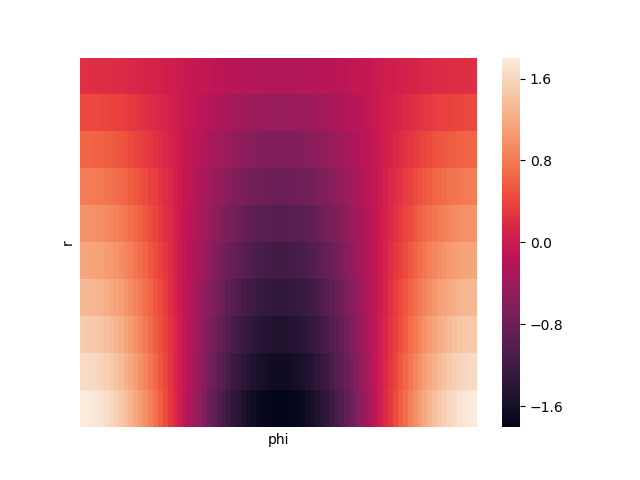
\includegraphics[width=0.9\textwidth]{Documentation/Figures/a06ex02c_uh.png} 
	\caption{}
	\label{fig:a05ex02b}
\end{figure}

The max error for the given $N_1$ and $N_2$ is 0.111, as 

\begin{figure}[H]
	\centering
	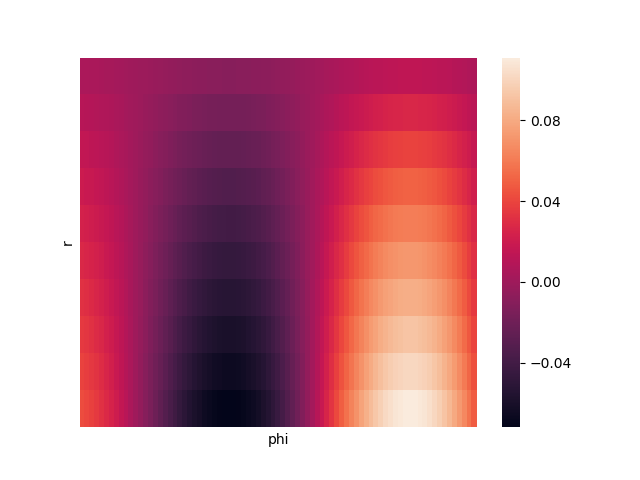
\includegraphics[width=0.9\textwidth]{Documentation/Figures/a06ex02c_error.png} 
	\caption{Error between the exact solution and the one obtained by the method in a). Notice the change in scale of the heat map}
	\label{fig:a05ex02b}
\end{figure}

\begin{figure}[H]
	\centering
	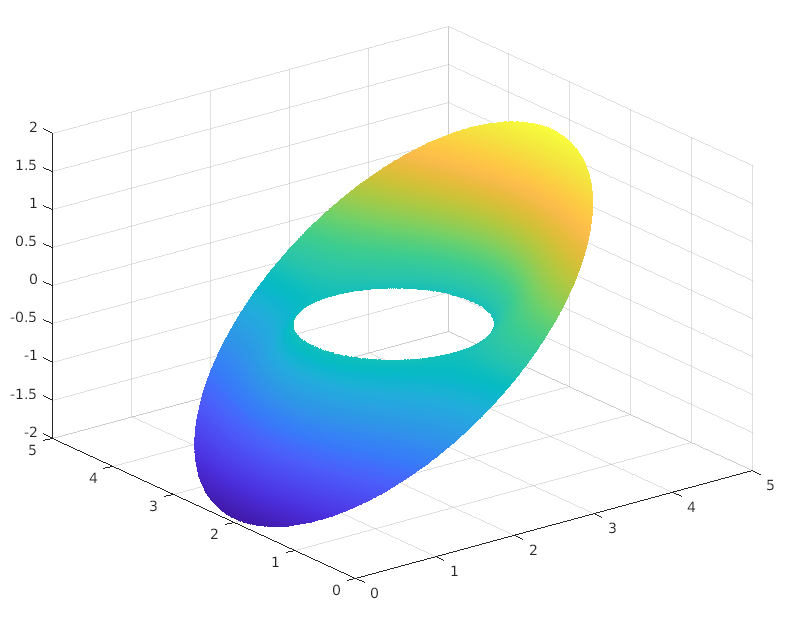
\includegraphics[width=0.9\textwidth]{Documentation/Figures/a06ex02d_uh.png} 
	\caption{Plot of the function values obtained using a modified version of the program from a05ex01}
	\label{fig:a05ex02b}
\end{figure}

\begin{figure}[H]
	\centering
	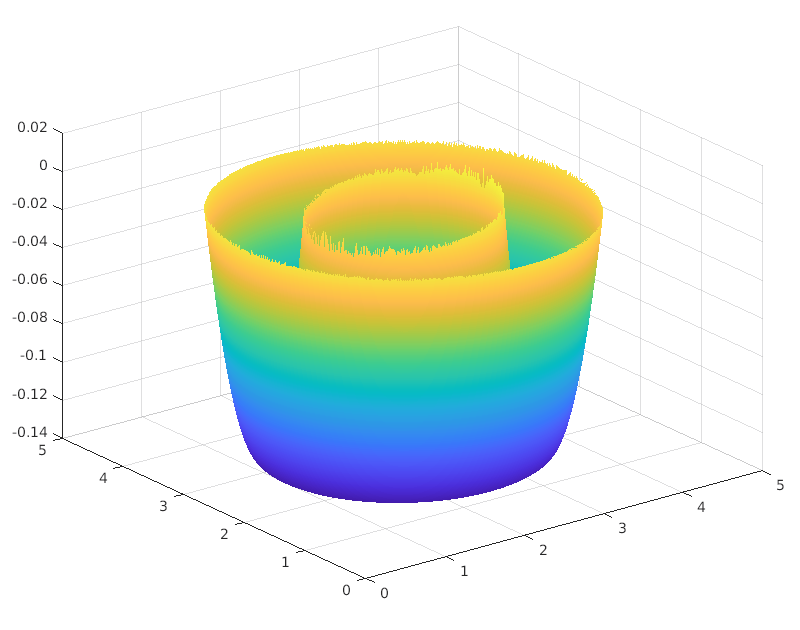
\includegraphics[width=0.9\textwidth]{Documentation/Figures/a06ex02d_error.png} 
	\caption{Error between the exact solution and the one obtained using a modified version of the program from a05ex01. Notice the change in scale of the vertical axis}
	\label{fig:a05ex02b}
\end{figure}